\documentclass{article}

% if you need to pass options to natbib, use, e.g.:
%     \PassOptionsToPackage{numbers, compress}{natbib}
% before loading neurips_2021

% ready for submission
% \usepackage[preprint]{neurips_2021}


% to compile a preprint version, e.g., for submission to arXiv, add add the
% [preprint] option:
%     \usepackage[preprint]{neurips_2021}

% to compile a camera-ready version, add the [final] option, e.g.:
\usepackage[final]{neurips_2021}

% to avoid loading the natbib package, add option nonatbib:
%    \usepackage[nonatbib]{neurips_2021}
\usepackage{authblk}

\usepackage[utf8]{inputenc} % allow utf-8 input
\usepackage[T1]{fontenc}    % use 8-bit T1 fonts
\usepackage{hyperref}       % hyperlinks
\usepackage{url}            % simple URL typesetting
\usepackage{booktabs}       % professional-quality tables
\usepackage{amsfonts}       % blackboard math symbols
\usepackage{nicefrac}       % compact symbols for 1/2, etc.
\usepackage{microtype}      % microtypography
\usepackage{xcolor}         % colors
\usepackage{tabularx}
\usepackage{graphicx}
\usepackage{caption}
\usepackage[cmex10]{amsmath}
\usepackage{amssymb}
\usepackage{amsthm}
\usepackage{CJKutf8}
\usepackage{xeCJK}

\title{TMALL Repeat Buyers prediction}

\author[1]{Armando Fortes}
\author[1]{David Pissarra}
\author[1]{Gabriele Oliaro}

\affil[1]{Department of Computer Science and Technology, Tsinghua University, Beijing, China \authorcr
  \{\tt ferreiracardos10, pissarrad10, oliarog10\}@mails.tsinghua.edu.cn}
  
  
\begin{document}

\maketitle

\begin{abstract}
  In this report, we describe a solution to the TMall Repeat Buyers Prediction challenge from the Tianchi portal on aliyun.com. We solved the machine learning problem as part of our final project for a Big Data Intelligence class at Tsinghua University. Our code performed well compared to the other submissions, placing us, at the time of our last submission (Dec 14, 2021), in the Top 40 among 6257 teams in total, or the top 0.6\%. 
\end{abstract}

\section{Introduction}
Promotions are a common way for vendors large and small to attract new buyers. It is especially common to offer discounts on particular shopping holidays such as on Nov.11 (Double 11 day) in China or on the Friday after Thanksgiving day (Black Friday) in the US. The idea is that some of the new buyers, initially visiting a store because of the lower prices, will then return as regular customers, thus allowing the store owners to earn back the money lost due the discounts, and make even more profits. Not all new customers, however, will be back when the undiscounted prices are restored, and so to maximize the return on investment (ROI), patrons need to design their promotion campaigns to target as exclusively as possible the people who are most likely to become loyal customers.

With the right amount of data, vendors can use machine learning tools to help solve the problem of optimizing the ROI of a promotion campaign. While this may not be feasible for small physical stores, putting together a large dataset with records on customer characteristics or the transaction details over a period of time, is feasible for large e-commerce platforms (such as TMALL), who are already likely to keep track of transactions and user info on a regular basis.

The competition \cite{tmall.com} provided us with a dataset (described in section \ref{dataset_section}) offered in two formats. The dataset was small enough (\textasciitilde 360MB) to allow training on commodity hardware. The dataset included a set of customer-vendor pairs without a label (indicating whether the customer had become a repeated buyer at the vendor's store). In order to obtain a position on the leaderboard, we had to submit a CSV file with our predictions (obtained through our machine learning model) for the pairs without a label. The competition website then computed the accuracy of our classifications, computed using a ROC AUC score, and ranked our submission by comparing our score with those obtained by the other teams.

After cleaning the data and performing normal preprocessing operations, we obtained our predictions in two main steps. First, we constructed the features that we were hoping would correlate most strongly with the output labels (section \ref{feature_engineering_section}). After having obtained the relevant features, we used a combination of gradient boosting (section \ref{boosting_section}) and a ensemble method (section \ref{ensemble_section}) to perform classification.

\section{The Dataset}\label{dataset_section}
The TMALL competition provided us with a dataset containing two main types of information:
\begin{enumerate}
    \item Customer demographic information, such as age and gender
    \item Customer-merchant interaction data:
    \begin{itemize}
        \item Label indicating whether the customer is a repeated buyer (training dataset) 
        \item Activity log: one record (with timestamp, category, brand and item number, plus the action type) for each item that was clicked, added to cart, purchased or added to favorite
    \end{itemize}
\end{enumerate}
To protect the buyers' and the vendors' privacy, the data was anonymized, and further is was also sampled in a biased way. 

The data is offered in two formats. The first format (file \texttt{data\_format1.zip}), divides the data in 4 tables, and it structured in a way that makes feature engineering easier. The second format (file \texttt{data\_format2.zip}) is more compact, as it consists of a single table, and minimizes the redundancy of information. Because our goal was to extract features, we picked format 1 (section \ref{dataset1_description}).

\subsection{The feature-engineering-ready dataset format}\label{dataset1_description}
The dataset from \texttt{data\_format1.zip} is organized in the following 3 tables: the User Profile Logs (Table \ref{tab:user_profile}), the User Behaviour Logs (Table \ref{tab:user_behavior_logs}), and the Training and Testing Data (Table \ref{tab:training_testing})

\begin{table}[htbp]
    \centering
    \setlength{\extrarowheight}{3pt}
    \begin{tabular}{|p{20mm}|p{75mm}|p{31mm}|}
        \hline
        \textbf{Data Field} & \textbf{Description} & \textbf{Data Type} \\
        \hline
        \texttt{user\_id} & The unique ID identifying each buyer & Integer \\
        \hline
        \texttt{age\_range} & The user's age range, encoded as follows: 1 for $<18$; 2 for $[18,24]$; 3 for $[25,29]$; 4 for $[30,34]$; 5 for $[35,39]$; 6 for $[40,49]$; 7 and 8 for $\geq 50$, 0 or NULL for unknown age, & Non-negative Integer or NULL\\
        \hline
        \texttt{gender} & The buyer's gender, encoded with 0 for female, 1 for male, 2 and NULL for unknown. & Integer or NULL \\
        \hline
    \end{tabular}
    \vspace{0.3cm}
    \caption{The User Profile Table}
    \label{tab:user_profile}
\end{table}
\vspace{-0.3cm}
\begin{table}[htbp]
    \centering
    \setlength{\extrarowheight}{3pt}
    \begin{tabular}{|p{20mm}|p{75mm}|p{31mm}|}
        \hline
        \textbf{Data Field} & \textbf{Description} & \textbf{Data Type} \\
        \hline
        \texttt{user\_id} & The unique ID identifying each buyer & Integer \\
        \hline
        \texttt{item\_id} & The unique ID identifying each possible item that can be bought & Integer \\
        \hline
        \texttt{cat\_id} & The unique ID identifying each possible category that an item can belong to & Integer \\
        \hline
        \texttt{merchant\_id} & The unique ID identifying each vendor & Integer \\
        \hline
        \texttt{brand\_id} & The unique ID identifying each brand an item can belong to & Integer \\
        \hline
        \texttt{time\_stamp} & The date (\texttt{mm}: month and \texttt{dd}: day) when an action took place & String in \texttt{mmdd} format\\
        \hline
        \texttt{action\_type} & The action taken by the buyer with respect to a vendor and an intem. Encoded as follows: 0 for a click, 1 for add-to-cart, 2 for purchase and 3 for add-to-favourite. & Integer \\
        \hline
    \end{tabular}
    \vspace{0.3cm}
    \caption{The User Behavior Logs Table}
    \label{tab:user_behavior_logs}
\end{table}

\begin{table}[htbp]
    \centering
    \setlength{\extrarowheight}{3pt}
    \begin{tabular}{|p{20mm}|p{75mm}|p{31mm}|}
        \hline
        \textbf{Data Field} & \textbf{Description} & \textbf{Data Type} \\
        \hline
        \texttt{user\_id} & The unique ID identifying each buyer & Integer \\
        \hline
        \texttt{merchant\_id} & The unique ID identifying each vendor & Integer \\
        \hline
        \texttt{label} & A binary value indicating whether \texttt{user\_id} became a repeated buyer at \texttt{merchant\_id}. Encoded as: 1 for repeat buyer, 0 for non-repeat buyer. The label is only available for the training portion of the data & Binary number (training), or empty (testing) \\
        \hline
    \end{tabular}
    \vspace{0.3cm}
    \caption{The Training and Testing Data Table}
    \label{tab:training_testing}
\end{table}

\vspace{1.5cm}

\section{Feature Engineering}\label{feature_engineering_section}
The given datasets, user\_log (user interation log) and user\_info (information about users) do not provide any structured features that can be directly embedded in some model. It turns out that these datasets need to be analyzed in order to create valuable features that can correlate users and merchants. We created some kinds of features which are going to be explained in detail throughout this section.

\subsection{Counting Features}
There are four types of actions between users and merchants: purchases, add-to-favourites, add-to-carts, and clicks. Each of these actions can be counted, creating an interesting set of features. For example, a user with a large amount of purchases on the last few months is very likely to buy anything in the future. In addition, we also count the actions of one user w.r.t. a specific merchant, or even the actions of all users with the merchant. Moreover, we calculate unique values existing on the dataset: categories, brands, dates, and others. Therefore, we are able to understand how many different brands were sold or bought from a merchant or user respectively. Over the previous counters, we could calculate some ratios, for instance the ratio between clicks and total number of actions.

\begin{table}[htbp]
    \centering
    \setlength{\extrarowheight}{3pt}
    \begin{tabular}{|c|c|c|c|c|c|}
        \hline
        \textbf{User ID} & \textbf{Items} & \textbf{Categories} & \textbf{Brands} & \textbf{Days} & \textbf{Months}\\
        \hline
        263947 & 36 & 26 & 20 & 22 & 6\\
        \hline
        338674 & 68 & 14 & 34 & 23 & 5\\
        \hline
        ... & ... & ... & ... & ... & ...\\
        \hline
        61119 & 153 & 46 & 72 & 34 & 4\\
        \hline
    \end{tabular}
    \vspace{0.3cm}
    \caption{Example of implemented counting features.}
    \label{tab:counters}
\end{table}
\vspace{-0.4cm}

In Table \ref{tab:counters}, it is denoted some examples of unique counted values. In this example the user with ID 263947 has bought 36 items from 26 different categories, 20 brands, on 22 different days, over 6 different months.

\subsection{Statistical Analysis Features}

Over the counting features which were previously mentioned, we calculate simple statistical analysis as follows:

\begin{itemize}
    \item Max – calculate the maximum value for a specific action regarding a user/merchant
    \item Mean – calculate the mean among action values for a given user/merchant
    \item Std – calculate the standard deviation over the action types for a user/merchant
    \item Median - calculate the median among action values for a given user/merchant
\end{itemize}

Despite the fact that these features seem quite simple, in fact 32 features were added to our dataframes, which really boosted our performance in the competition.

\subsection{Time Span Features}

The given dataset has information about interactions between users and merchants along 186 days (from 11 May to 12 November). Therefore, we could divide this big dataset into 6 smaller periods of time, each of them with exactly 31 days, as shown in Figure \ref{fig:time}.

\begin{figure}[h!]
    \centering
    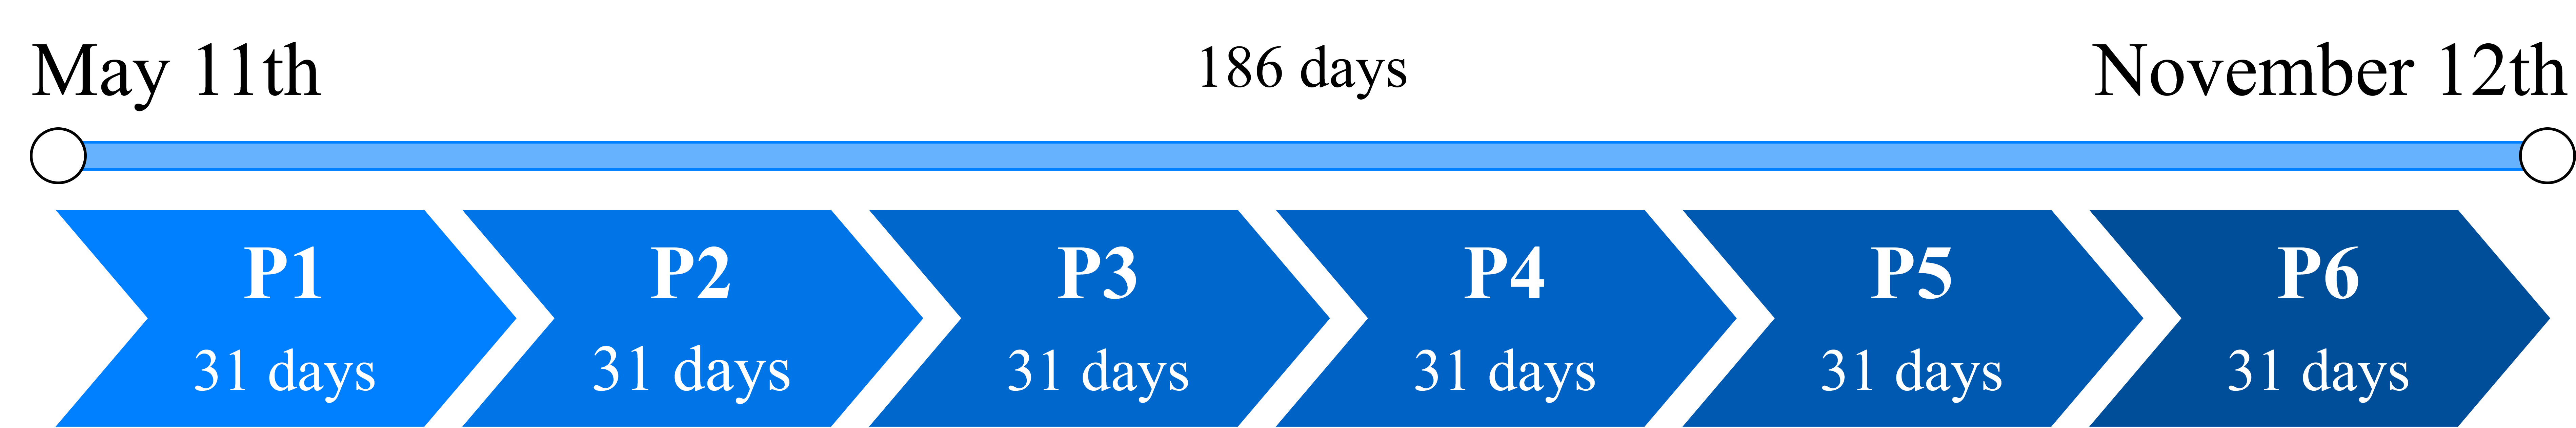
\includegraphics[width=0.9\linewidth]{figs/time.png}
    \vspace{0.1cm}
    \caption{Dataset time span.}
    \label{fig:time}
\end{figure}

Each of these periods was respectively analyzed by fetching counting features for each period over all kinds of actions. Additionally, we calculated for each of 4 actions the slope of the linear regression function regarding the time periods (Equation \ref{eq:trend}). Therefore, we can calculate if some user is buying more products over the time (Figure \ref{fig:user}), which may represent that this user is likely to buy more products in the meantime. On the other hand, if there is, for example, a merchant which is getting less clicks period by period, it might point out that this merchant will lose some costumers.

\begin{align} \label{eq:trend}
    \frac{n \sum x y - (\sum x) (\sum y)}{n (\sum x^2) - (\sum x)^2}
\end{align}

\begin{figure}[h!]
    \centering
    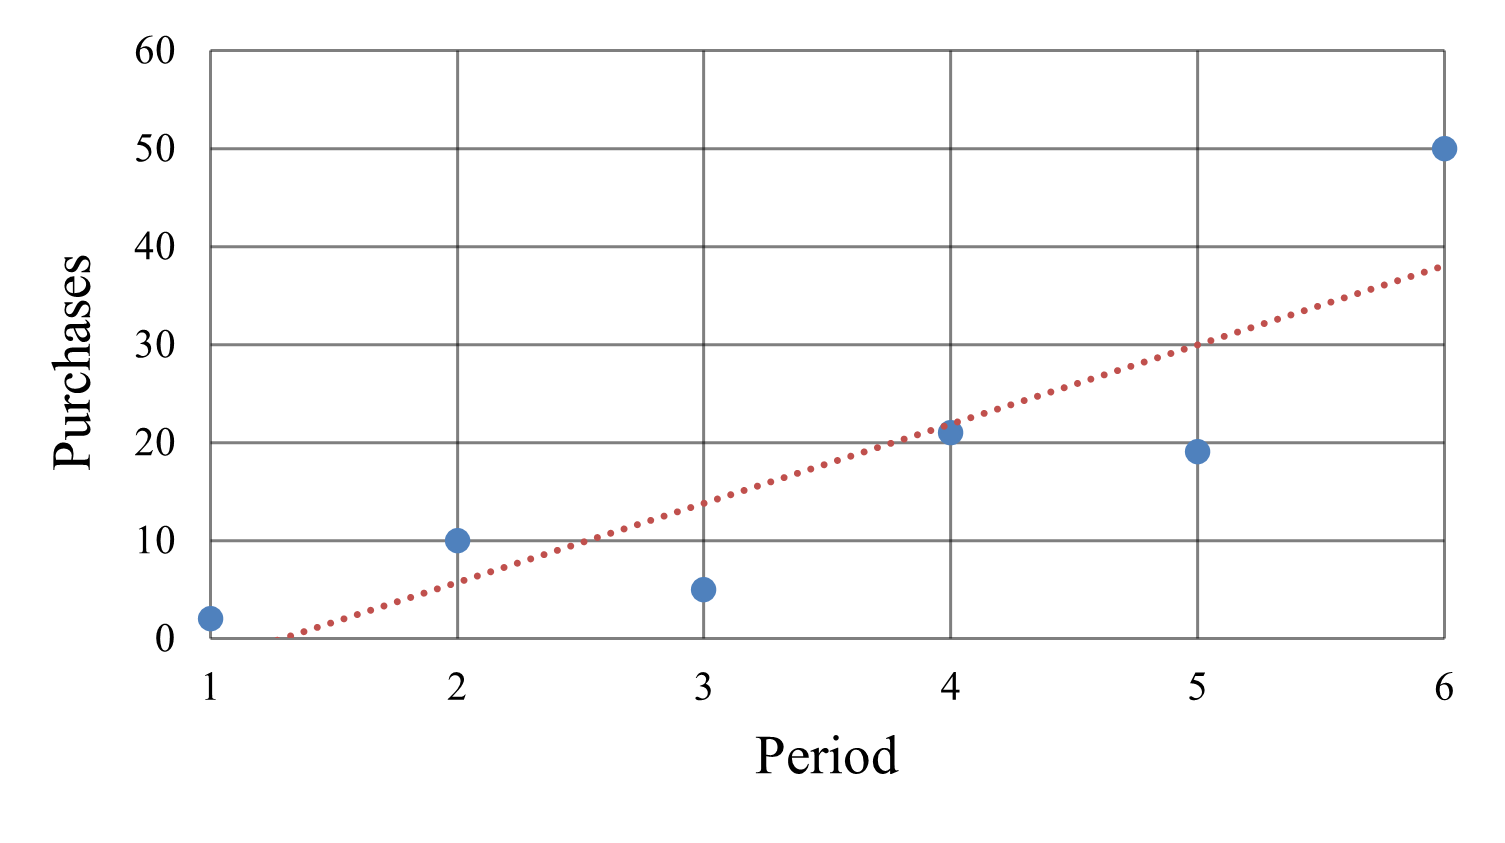
\includegraphics[width=0.65\linewidth]{figs/user.png}
    \caption{User uptrend example.}
    \label{fig:user}
\end{figure}

\subsection{Double 11 Features}

Double 11 is a very popular shopping festival in China, leading to huge volumes of transactions. As shown on Figure \ref{fig:double11}, there is a big amount of interactions when compared to the remaining 185 days. Hence, we counted values and calculated ratios over the number of actions for each user, merchant, and aggregation user-merchant. People that purchase products on days like this may only take advantage of big promotions, being one-time deal hunters.
\vspace{-0.3cm}
\begin{figure}[h!]
    \centering
    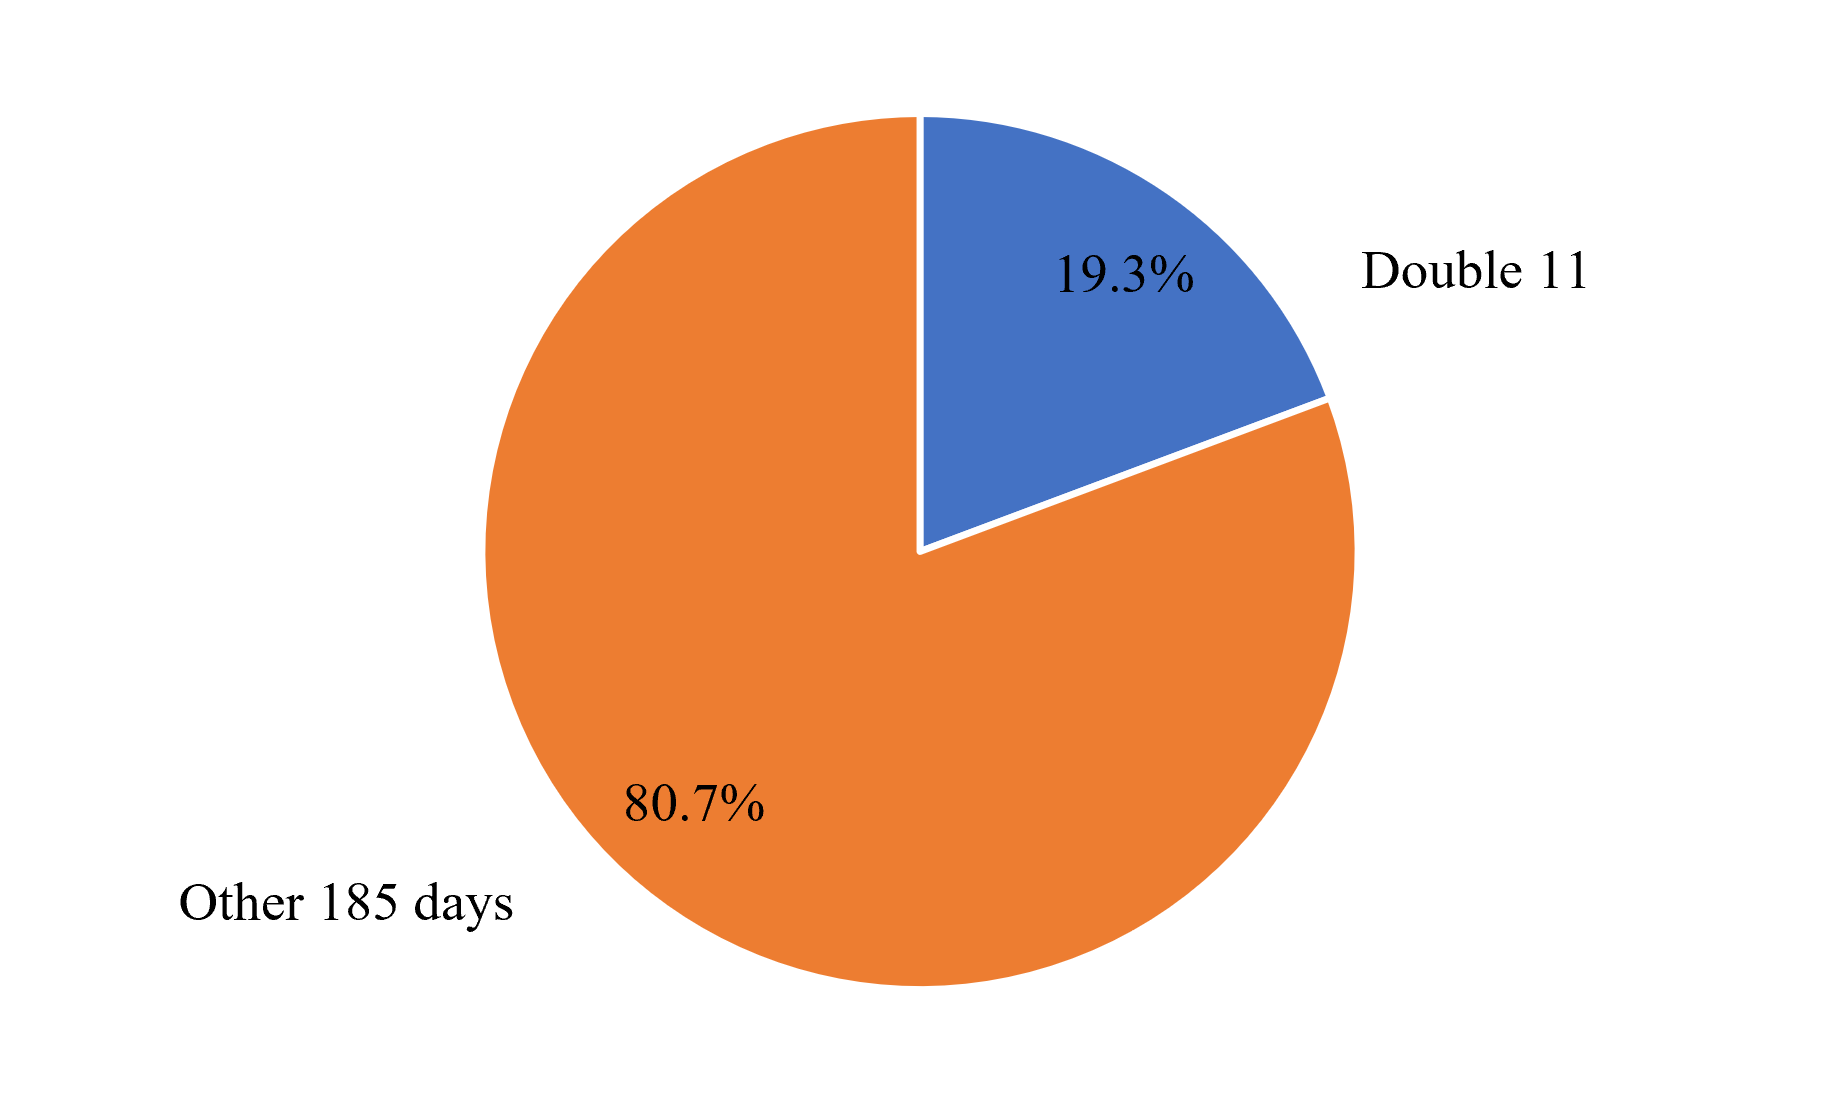
\includegraphics[width=0.65\linewidth]{figs/double11.png}
    \caption{Double 11 impact on the dataset.}
    \label{fig:double11}
\end{figure}

\vspace{4cm}

\subsection{Principal Component Analysis Features}

With the previous described features, we created 285 features in total. However, we summarize our dataframe by using Principal Component Analysis (PCA) in a smaller number of features (5 components, which can be seen as an hyperparameter). These 5 PCA features will be added to the entire dataset giving more useful data to the inference. By using PCA we will create 5 new features that increase the interpretability by maximizing the variance, so the model will better distinguish patterns of users or merchants. To conclude, we end up creating 290 features that will be received by our model.

\section{Method}\label{method_section}

\subsection{Gradient Boosting}\label{boosting_section}

Gradient Boosting is a very famous technique, which of course comes from the concept of Boosting, where we try to improve single weak models (in this case, decision trees) by combining them together, in order to generate a collectively strong model. Moreover, it actually extends the Boosting concept, since the addition of the generated weak models is formalized as a Gradient Descent algorithm, over an objective function. Also, each of the decision trees is added one at a time, and trained using the residual errors of their predecessors as labels, therefore, at each iteration, the focus is directed to the samples which have not yet been accurately predicted.\\
After thorough research for implementations of the Gradient Boosting technique, we found that XGBoost \cite{xgboost}, LightGBM \cite{lightgbm} and CatBoost \cite{catboost} were some of the best ones for this type of problem. They are usually able to achieve great results, specially XGBoost which is the most used Gradient Boosting implementation for tabular data, regarding Kaggle competition winning solutions. Consequently, we decided integrate them and see how they would perform on the features we had developed.

\subsection{Ensemble} \label{ensemble_section}

At First, we relied on XGBoost \cite{xgboost} to make our predictions in the competition, since it was the model with the best results in our 10-Fold Cross Validation (section \ref{subkfold}). However, we decided to build an Emsemble Model which would take into account the predictions from every individual implementation, because, even though XGBoost had the best performance so far, perhaps the other models were also extracting useful signals from the data that would complement the ones of XGBoost. Accordingly, we used Equation \ref{ensemble}, where we assign a weight to each model and calculate the corresponding weighted average for our predictions.\\
\begin{align} \label{ensemble}
    P(u, m) = \sum_K w_k \cdot P_k(u, m)\textrm{, \> where} \sum_K w_k = 1
\end{align}\\
We started by assigning weights according to the performance of each model during cross validation, so XGBoost would have the largest weight, and so on. After manually tuning the weights, we were able to find an optimal combination and achieve improved results, which are presented in the following section.

\section{Evaluation and Experiments}
\subsection{The ROC AUC score}
The ROC AUC score is an evaluation metric used to benchmark all submissions to the TMALL Repeat Buyers Prediction. ROC AUC stands for Area Under the Curve (AUC) of the Receiver operating characteristic (ROC) graph.\\
The ROC graph is a curve with the specificity (or probability of obtaining false positives in the classification) as the independent variable and the sensitivity (or probability of obtaining true positives in the classification) as the dependent variable. To obtain the curve, we compute the FPR (false positive rate) and the TPR (true positive rate) at several threshold settings, then plot the data points obtained.\\
Given the ROC plot, the AUC is simply the area between the ROC curve and the x-axis (i.e. the specificity axis). It can be computed simply by taking the integral of the ROC curve. Higher values of the AUC indicate better classifiers, because larger areas under the ROC curve are obtained if the curve is made up of points whose y-axis value are larger (i.e. the TPRs are larger).

\subsection{K-Fold Cross Validation} \label{subkfold}

After selecting the three Gradient Boosting implementations, we decided to run K-Fold Cross Validation on each of the models. This method consists in dividing our dataset into K splits and using one of these splits as a validation set, while the others serve as training. This is performed for every possible combination of splits. Accordingly, we are able to estimate the skill of the machine learning models, since we are exposing them to various different combinations of splits for training and validation. We used 10 folds and achieved the results presented in Table \ref{tab:score}. 

\begin{table}[h!]
\centering
\setlength{\extrarowheight}{3pt}
\begin{tabular}{|c|c|}
    \hline
    \textbf{Model} & \textbf{ROC-AUC Score}\\
    \hline
    XGBoost & 0.6916\\
    \hline
    LightGBM & 0.6773\\
    \hline
    CatBoost & 0.6871\\
    \hline
    \textbf{Ensemble Model} & \textbf{0.6924}\\
    \hline
\end{tabular}
\vspace{0.3cm}
\caption{10-fold cross validation average results of the different implementations.}
\label{tab:score}
\end{table}
\vspace{-0.4cm}

In terms of individual implementations, XGBoost \cite{xgboost} had the best results, followed by CatBoost \cite{catboost}, and finally LightGBM \cite{lightgbm}. However, as previously mentioned, the Ensemble Model managed to outperform all the others, by combining their predictions.

\subsection{Best Feature Fetching}

One further experiment we added to our study was to use the XGBoost \cite{xgboost} algorithm to calculate how important each feature we implemented actually is. For this purpose, XGBoost analyzed the improvement in accuracy brought by each feature to the branches it is on. Afterwards, we were able to sort the features by importance and select only the most important ones for training. Some of the most important features developed, according to XGBoost, are presented in Table \ref{tab:fetimportance}.\\
Upon filtering the most important features, we went from 290 to 150, which corresponds to almost a 50\% cut. With this procedure we intended to analyze which of the developed features had the greatest influence in our results, and potentially decrease the complexity of the learning process, without affecting performance.

\vspace{2cm}

\begin{table}[h!]
\centering
\setlength{\extrarowheight}{3pt}
\begin{tabular}{|c|c|}
    \hline
    \textbf{Feature} & \textbf{Importance}\\
    \hline
    items\_user\_merchant & 5.3590\\
    \hline
    purchases\_user\_merchant\_period\_5 & 5.2504\\
    \hline
    purchases\_user\_merchant & 5.1866\\
    \hline
    categories\_user\_merchant & 4.0474\\
    \hline
    periods\_user\_merchant & 4.0189\\
    \hline
    double11\_periods\_user\_merchant\_ratio & 2.9512\\
    \hline
    ... & ...\\
    \hline
\end{tabular}
\vspace{0.3cm}
\caption{Features sorted by importance.}
\label{tab:fetimportance}
\end{table}
\vspace{-0.3cm}

\begin{table}[h!]
\centering
\setlength{\extrarowheight}{3pt}
\begin{tabular}{|c|c|c|}
    \hline
    \textbf{Model} & \textbf{Every Feature} (290) & \textbf{Best Features} (150)\\
    \hline
    XGBoost & 0.6913 & 0.6916\\
    \hline
    LightGBM & 0.6773 & 0.6757\\
    \hline
    CatBoost & 0.6871 & 0.6882\\
    \hline
    \textbf{Ensemble Model} & 0.6924 & \textbf{0.6925}\\
    \hline
\end{tabular}
\vspace{0.3cm}
\caption{ROC-AUC scores of the different implementations before and after best feature fetching.}
\label{tab:scorebest}
\end{table}
\vspace{-0.3cm}

As one may observe in Table \ref{tab:scorebest}, fetching the best features was not a huge improvement on performance, however, it successfully reduces the complexity of learning process as well as the time taken by each model to be trained, while still maintaining top results. In the end, our best model is again the Ensemble model, trained using only the 150 best features.

\section{Conclusion}
In this project, we successfully tackled the TMALL Repeat Buyers prediction challenge by Aliyun.com, placing ourself among the Top 40 teams on the Leaderboard, at the time of submission. As of today (Jan 4, 2021), after more than 250 additional teams submitted their solutions, our Dec. 14 submission still ranks \#45 out of a total of 6524 teams, or in the top 0.68\% of all submissions. Our team name was \texttt{davidpissarra} and affiliation: \texttt{\begin{CJK*}{UTF8}{gbsn}清华大学\end{CJK*}}.

To achieve this result, first, we spent a significant amount of time performing feature engineering, in order to organize the information in the data in a way that allowed our classifier models to be most effective. We then designed a classifier architecture based on boosting, and computed our final results using an ensemble model based on XGBoost \cite{xgboost}, LightGBM \cite{lightgbm} and CatBoost \cite{catboost}. 

\bibliography{references}
\bibliographystyle{IEEEtran}

\end{document}